\documentclass{IEEEtran}
\usepackage{savesym}
\usepackage[thinlines,thiklines]{easybmat}
\usepackage{etex}
%\usepackage{psfrag}
\usepackage{amsmath}
\usepackage{amssymb}
%\usepackage{mathabx}
%\usepackage{mathrsfs}
\usepackage{graphicx}
\usepackage{epstopdf}
\usepackage{subfigure}
\usepackage{verbatim}
\usepackage{array}
\usepackage{latexsym}
\usepackage[dvipsnames]{xcolor}
\usepackage{cite}
\usepackage{stmaryrd}
%\usepackage[numbers,sort&compress]{natbib}
\usepackage{multirow}
%\usepackage{subequation}
\usepackage{textcomp}
%\usepackage[center]{caption}
%\usepackage{ful\subsubsection{Decoupled single cluster approach}
\usepackage[ruled,linesnumbered,algoruled,boxed,lined]{algorithm2e}
\usepackage{algorithmic}
\usepackage{bm}
\usepackage[left=0.75in,top=0.72in,right=0.75in,bottom=0.78in]{geometry}
\AppendGraphicsExtensions{.pdf}
\graphicspath{{new_figs/}}
\usepackage{booktabs}
\usepackage{adjustbox}
\savesymbol{comment}
%\usepackage{changes}
\usepackage{caption}
\usepackage{subcaption}
\SetKw{Continue}{continue}
\SetKwBlock{Repeat}{repeat}{}

\restoresymbol{CHG}{comment}
\newcommand{\var}[1]{\text{\texttt{#1}}}
\newcommand{\func}[1]{\text{\textsl{#1}}}

\graphicspath{{figs/}}



\begin{document}
	\title{A motion planning and motion control framework for autonomous vehicles}

\begin{abstract}
	In this project, we present a motion planning and motion control framework for aggressive driving of an autonomous vehicle, with the aim of obtaining an time-optimal trajectory. The framework consists of four major works: (i) a sampling-based planner, (ii) a novel path smoothing method, (iii) a trajectory optimization procedure on a track formed by smoothed path, and (iv) a trajectory tracking process. A sampling-based planner called $\tt Bi-iSST$ is proposed to quickly generate time-optimal trajectories for autonomous driving scenario by utilizing the bidirectional approach to speed up the searching process, and avoiding solving boundary value problem. A classic smoothing approach first is applied on the path generated by the sampling-base planner, without the consideration of the dynamics and the initial orientation. Then the smoothed path is treated as a beam with supports on both ends and pre-defined stretch. Two kinds of virtual force are applied on the beam: (i) force due to the virtual potential emitted by obstacles and (ii) torques force the beam flat if the curvature exceeds minimal turning radius. After the smooth process is finished, the beam is fitted by a special parametric spline and used as the center-line of a race track in the third stage. Finally an optimization strategy is employed to get a trajectory with minimal traveling time and an MPC is applied to track this trajectory. 
	Another sampling-based planning algorithm called $\tt Ref$-$\tt iSST$ is also developed for wireless external actuation micro-scale wire control system. A transition matrix similar to that in Markov Decision Processes is used to form the reference trajectory.
\end{abstract}

\section{Introduction}
The last three decades have seen steadily increasing research efforts, both in academia and in industry, towards developing driverless vehicle technology. Driverless cars are essentially autonomous decision-making systems that process a stream of observations from on-board sensors such as radars, LIDARs, cameras, GPS units, and odometry. These observations, together with prior knowledge about the road network, rules of the road, vehicle dynamics, and sensor models, are used to automatically select values for controlled variables governing the vehicle’s motion. Intelligent vehicle research aims at automating as much of the driving task as possible. These developments have been fueled by recent advances in sensing and computing technology. The automotive engineers today face the challenge of designing autonomous safety systems that can utilize the full capabilities of the vehicle’s tires in emergency scenarios to avoid accidents and significant understeer or oversteer. % These extremely agile driving skills motivate the design of autonomous control for safe, unstable vehicle motion under extremely events.  

The decision making in contemporary autonomous driving systems is typically hierarchically structured into route planning, behavioral decision making, local motion planning band feedback control. The partitioning of these levels are, however, rather blurred with different variations of this scheme occurring in the literature. This research focus on these core problems of autonomous aggressive driving. Particular emphasis is placed on methods for motion planning and control. 
\begin{figure}
	\subfigure[]{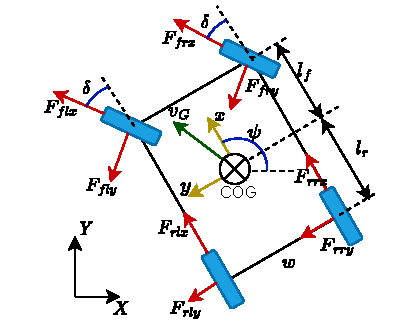
\includegraphics[width=0.4\textwidth]{fig_4_wheel}\label{fig:4_wheel}}
	\subfigure[]{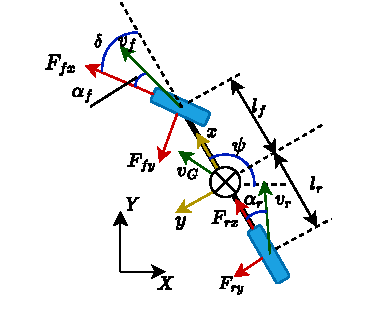
\includegraphics[width=0.4\textwidth]{fig_2_wheel}\label{fig:2_wheel}}
	\label{fig:three graphs}
	\caption{Schematics of the vehicle dynamics modeling configuration. \newline  (a) 4 wheel model; (b) 2 wheel model}
\end{figure}
\section{Problem Statement}
The primary focus of this project is to develop a motion planning algorithm to find a feasible, smooth and optimal trajectory within an acceptable time for an autonomous vehicle, by utilizing the extreme performance of a vehicle, as well as a motion control algorithm that allows the vehicle to drive at the handling limits with the same capability as a professional race driver. 
\subsection{Vehicle Model}
We consider an all-wheel steering vehicle on the horizontal plane and Fig.\ref{fig:4_wheel} illustrates the schematic of the vehicle modeling configuration. A ground-fixed frame $\mathcal{N}(X,Y)$ and a body-fixed frame $\mathcal{N}(X,Y)$ are used to build the model. The origin of $\mathcal{B}(x,y)$ is located at the vehicle mass center (denoted as $COG$).
The longitudinal and lateral forces are denoted as $F_{ijx}$ and $F_{ijy}$, $i=f, r$ and $j=l,r$, at the front (rear), left (right) wheels, respectively. Denoting the steering angle as $\delta$, the equations of motion of the vehicle are obtained as:
\begin{equation}\label{4_wheel_model}
	\begin{aligned}
		m\dot{v_x} & = F_{rlx}+F_{rrx}+(F_{flx}+F_{frx})\cos(\delta) \\
		 & -(F_{fly}+F_{fry})\sin(\delta)+mv_y\dot\psi \\
		m\dot{v_y} & = F_{rly}+F_{rry}+(F_{flx}+F_{frx})\sin(\delta) \\ 
		& +(F_{fly}+F_{fry})\cos(\delta)-mv_x\dot{\psi}\\
		I_z\dot{\omega} & = \left[(F_{fly}+F_{fry})\cos(\delta)+(F_{flx}+F_{frx})\sin(\delta))\right]l_f \\
		& -(F_{rly}+F_{rry})l_r + \frac{w}{2}[(F_{frx}-F_{flx})\cos(\delta) \\ 
		& +(F_{fly}-F_{fry})\sin(\delta)+(F_{rrx}-F_{rlx})]
	\end{aligned}
\end{equation}
Due to the symmetry of vehicle along the longitudinal center line, the model is simplified to a bicycle model. By introducing the vehicle yaw speed $\omega$ and steering speed $\delta_{\tt dot}$, the Eq.(\ref{4_wheel_model}) can be written as:

\begin{subequations}\label{2_wheel_model}
	\begin{align}
	\dot{X}  & = v_x \cos(\psi)-v_y \sin(\psi)\\
	\dot{Y} & = v_x \sin(\psi)+v_y \cos(\psi) \\
	\dot{\psi} & = \omega \\
	\dot{v_x} & = \frac{1}{m}\left(F_{r,x}+F_{f,x}\cos(\delta)-F_{f,y}\sin(\delta)+mv_y\omega\right)\\
	\dot{v_y} & = \frac{1}{m}\left(F_{r,y}+F_{f,x}\sin(\delta)+F_{f,y}\cos(\delta)-mv_x\omega\right)\\
	\dot{\omega} & = \frac{1}{I_z}\left((F_{f,y}\cos(\delta)+F_{f,x}\sin(\delta))l_f-F_{r,y}l_r\right) \\
	\dot{\delta} & = \delta_{\tt dot}
	\end{align}
\end{subequations}
Rewrite Eq.(\ref{2_wheel_model}) to
\begin{equation}
	\dot{x} = f(x,u)
\end{equation}
where $x \in \mathcal{X}$ is the state, belonging to a n-dimensional manifold $\mathcal{X}$(the state space), and $u=[\delta_{\tt dot},F_{f,x},F_{r,x}]^T$ is the control input. The preceding formulation can include both nonholonomic and dynamic constraints. 

The vehicle uses rubber tires and the motion heavily depends on the tire-road interaction forces. The longitudinal friction forces are functions of the slip ratios, namely, $F_{i,x} = \mu_x F_{i,z},i=f,r$ where $\mu_x$ is the longitudinal friction coefficient, which is a function of the longitude slip ratios $\lambda_i$. Similarly, The lateral friction forces are functions of the slip angle, namely, $F_{i,x} = \mu_y F_{i,z},i=f,r$ with lateral friction coefficient $\mu_y(\alpha_i)$, where $\alpha_i,i=f,r$ are the slip angles shown as in Fig.\ref{fig:2_wheel}.

\subsection{Motion Planning}
The motion-planning problem can be stated as follows: given an initial state $x_0 \in \mathcal{X}$ , at time $t_0$, and a goal equilibrium configuration $x_f$, find a set of control inputs $ u:[t_0; t_f] \rightarrow \mathcal{U}$ that can drive the agent from $x_0$ to $x_f$. Although the usual formulation of the motion-planning problem is concerned only with finding a feasible trajectory, in this project we are also interested in finding a trajectory minimizing the traveling time.

Sampling-based motion planners, such as the rapidly exploring random tree (RRT) and its variants, are widely
applied for great efficiency at generating a trajectory.
RRTs take sample points in the search space and add them
to a tree that covers the whole space with probabilistic
completeness. However, the RRT method is not optimal.
Although the RRT* algorithm can be asymptotically
optimal, its convergence is slow for large scale problems. 

\subsection{Motion Control}
In order to execute the reference path or trajectory from the motion planning system a feedback controller is used to select appropriate actuator inputs to carry out the planned motion and correct tracking errors. The tracking errors generated during the execution of a planned motion are due in part to the inaccuracies of the vehicle model. Thus, a great deal of emphasis is placed on the robustness and stability of the closed
loop system.
Many effective feedback controllers have been proposed
for executing the reference motions provided by the motion planning system to stabilize the reference path or trajectory in the presence of modeling error and other forms of uncertainty. Depending on the reference provided by the motion planner, the control objective may be path stabilization or trajectory stabilization.


Model predictive control is a general control design
methodology which can be very effective for autonomous driving. Conceptually, the approach is to solve the motion planning problem over a short time horizon, take a short interval of the resulting open loop control, and apply it to the system. While executing, the motion planning problem is re-solved to find an appropriate control for the next time interval. Advances in computing hardware as well as mathematical programming
algorithms have made predictive control feasible for real-time use in driverless vehicles. 


\section{Completed Work}

Fig.\ref{fig:framework} shows an overview of the motion planning and tracking scheme of the project. Different from other frameworks which use the path directly from sampling-based algorithm (and a smooth process) as the reference trajectory, in the framework of this project, the smoothed path is used as the centerline of a racetrack, and an optimization process called Minimum-Lap-Time is applied to get a time-stamped optimal trajectory on this road. It is a big challenge to get the optimal control input sequence for a racing car due to its high speed and nonlinear behavior of the high fidelity model. 

\begin{figure}[h]
	\centering
	\captionsetup{justification=centering}
	\scalebox{0.8}{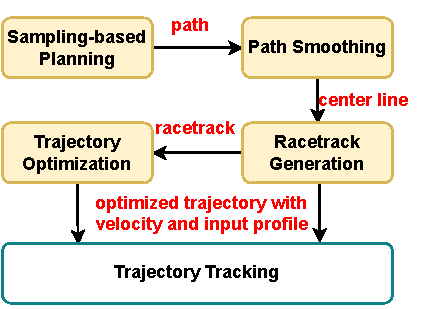
\includegraphics{framework.pdf}}
	\caption{Path Planning Framework}
	\label{fig:framework}
\end{figure}
\subsection{Bi-Directional Sparse Stable Sampling-Based Algorithm}
The rapidly exploring random tree algorithm ($\tt RRT$)\cite{lavalle1998rapidly} samples in state space, then tries to connect the sampled state to the nearest node on the tree by solving a boundary value problem (BVP). The Stable Sparse RRT($\tt SST$)\cite{sst} samples on input space to avoid such extra computational cost, especially for agents with high state space dimensions. However, sampling in input space breaks the uniform distribution in state space, leading to a lot of redundant samplings. To solve this problem, an additional set, $\mathbb{W}$, is employed in SST to monitor the sampling states, to make sure in a certain region only one node, which has least cost from the start state (in most cases it refers to the traveling time), is active at most. Any new state located in this region has to compare the cost with this active node. The states with higher cost will be ignored. 

The bidirectional informed $\tt SST$, ${{\tt Bi}}$-${{\tt iSST}}$, is developed for this project. Algorithm~\ref{biisst} shows the structure of the ${{\tt Bi}}$-${{\tt iSST}}$ algorithm. Compared with the ${{\tt SST}}$ algorithm, the ${{\tt Bi}}$-${{\tt iSST}}$ algorithm maintains two trees, $\mathcal{G}_{\tt a} $ and $ \mathcal{G}_{\tt b} $, as well as their witness sets, $\mathbb{W}_{\tt a} $ and $ \mathbb{W}_{\tt b} $. The roots of the two trees are on the start state and the target state of all the agents, respectively (Line 1). A tree is randomly selected to propagate by following the $\tt iSST$ propagation as described in Algorithm~\ref{isst_step}, which generates a set of new vertices $\mathbb{X}$.

A set $\mathbb{P}$ is maintained to collect the vertices that are near to any vertex whose distance to the other tree is below $\delta_{\tt watch}$. A process is employed to connect the vertices in $\mathbb{P}$ to the other tree, to accelerate the path finding speed. 

\begin{algorithm}[ht!]
	\caption {${{\tt Bi}}$-${{\tt iSST}}$}
	\label{biisst}
	% \Input{ $\textbf{q}_{\tt s},\textbf{q}_{\tt t}$}
	% \Output{ $\mathcal{G}_{\tt a},\mathcal{G}_{\tt b}$}
	\DontPrintSemicolon
	\SetAlgoVlined
	\BlankLine
	
	$\mathcal{G}_{\tt a},\mathbb{W}_{\tt a} \gets \mathtt{init}(\textbf{q}_{\tt s})$, $\mathcal{G}_{\tt b},\mathbb{W}_{\tt b} \gets \mathtt{init}(\textbf{q}_{\tt t})$, $\mathbb{P} \gets \emptyset$\;
	
	\For{$m\ \text{iterations}$}{	
		
		$u \gets {\tt Uniform}([0,1])$ \;
		\uIf{$u<0.5$}{
			$\mathbb{X} \gets \mathtt{iSST\_Propagation}(\mathcal{G}_{\tt a},\mathbb{W_{\tt a}},\textbf{q}_{\tt t})$ \;
			$\mathcal{G'} \gets \mathcal{G}_{\tt b}$
		}
		\Else{
			$\mathbb{X} \gets \mathtt{iSST\_Propagation}(\mathcal{G}_{\tt b},\mathbb{W_{\tt b}},\textbf{q}_{\tt s})$ \;
			$\mathcal{G'} \gets \mathcal{G}_{\tt a}$
		}
		\ForEach{$x \in \mathbb{X}$}{			
			$x_{\tt closest} \gets \mathtt{Closest\_Node}(\mathcal{G'},x)$\;
			\If {$\mathtt{distance}(x,x_{\tt closest})<\delta{_{\tt watch}}$}{
				$\mathbb{P} \gets \mathbb{P} \cup \{x\}$\;
				%$\mathrm{Optimized\_Connection()}$\;
			}
			%			\lElse{	$\mathcal{G'}.\mathbb{O} \gets \mathcal{G'}.\mathbb{O} \cup \{x\}$	}
		}
	}

	%	\Return{ $\mathcal{G}_{\tt a},\mathcal{G}_{\tt b}$}
	
\end{algorithm}



\begin{algorithm}[ht!]
	\caption {${\tt iSST\_Propagation}$}
	\label{isst_step}
	% \Input{ $\mathcal{G},\mathbb{W},\bs{q}$}
	% \Output{ $\mathbb{X}$}
	\DontPrintSemicolon
	\SetAlgoVlined
	\BlankLine	
	
	$x_{\tt curr} \gets \mathtt{Search\_Selection}(\mathbb{O},\mathbb{O'})$, $\mathbb{X} \gets \emptyset$\;		
	\While {True}{
		$x_{\tt new} \gets \mathtt{Blossom}(x_{\tt curr},q)$\;
		\If {$ {\tt not } \  \mathtt{Collision\_Free}(\overline{x_{\tt curr}\rightarrow x_{\tt new}})$ }{
			\Return
		}
		\If {$ {\tt not}\  \mathtt{Local\_Best\_SST}(x_{\tt new},\mathbb{W},\delta_{\tt s})$ }{
			\Return
		}
		$\mathbb{X} \gets \mathbb{X} \cup x_{\tt new}$, $\mathbb{V}_{\tt active} \gets \mathbb{V}_{\tt active} \cup \{x_{\tt new}\}$\;
		$\mathbb{E} \gets \mathbb{E} \cup \{\overline{x_{\tt curr}\rightarrow x_{\tt new}}\}$\;
		$\mathtt{Prune\_Dominated\_Nodes\_SST}(\mathcal{G},\mathbb{W},x_{\tt new})$\;
		$x_{\tt curr} \gets x_{\tt new}$				
		
	}
\end{algorithm}



% \begin{eqnarray}	
% 	\min_{\textbf{u}_c} &J  &= \int_0^{c_{\tt conn}} 1 \text{d} t \label{BVP}\\
% 	\tt{subject to}  &\dot{\textbf{q}}(t) &=\textbf{\textit{\Theta}}\textbf{B}(\textbf{q}(t))\textbf{u}_c(t) \nonumber\\
% 	&\textbf{q}(0) &= x_{\tt p}.\textbf{q}, \quad\textbf{q}(c_{\tt conn})= x_{\tt p}.\textbf{q} \nonumber
% 	\label{optbvp}
% 	\end{eqnarray}

\subsection{Trajectory Smoothing}
Several sampling-based motion planners are able to output an optimal trajectory\cite{sst}\cite{anytimemotion}. However, massive computation time is required to achieve such optimal trajectory. For real applications, the time for planners is limited, causing jerky output paths which are less human-friendly. Typically, the output of the sampling-based planner should be smoothed, in most case of which the dynamics feasibility will not be maintained. So to accelerate the computation, the simple kinematic model is adopted in the sampling-base stage, and the more complex dynamics model is considered in the late procedures to exploit the maximum performance of the vehicle.

Most of the existing path smoothing methods are not applicable for car-like robot since the initial orientation is not considered, causing the smoothed path unreachable. The proposed approach here aims at solving such phenomenon and to generate a more natural path. For example the Convex Elastic Smoothing (CES)\cite{zhu2015convex} algorithm (CES) algorithm uses the following strategy:
\begin{subequations}\label{ces}
	\begin{align}
		\min \quad & \sum \|D_{i+1}-D_{i}\|_2^2\\
		\textrm{s.t.} \quad & D_{k}=\pi_{i}-\pi_{i-1},\pi_1 = Q_1,\pi_n = Q_n\\
		\quad &  \pi_i \in \mathcal{B}_i ,\|D_{i+1}-D_{i}\| \leqslant \frac{d^2}{R_{\tt min}} \\
		\quad & \pi_2 = P_1 + k\frac{Q_2-Q_1}{\|Q_2-Q_1\|} \label{ces_direction}
	\end{align}
\end{subequations}
Where $\mathcal{B}$ is a collision-free tube along the original trajectory $Q$, and $\pi$ is the smoothed path.
Eq.(\ref{ces_direction}) is used to control the initial orientation of the smoothed path. However, in this case, the sharp turn may appear at the second segment $D_2$ sometimes. 

Consider the trajectory from sampling-based method as a Bernoulli-Euler~\cite{Truesdell1984} beam with some external forces and pre-defined deformations, as well as constraints on the two ends. The dynamics deforming process due to such forces and deformations is equivalently treated as the path smoothing process. Now take the dynamic analysis of the beam by deriving its equations of motion(EOMs) to get the variation of displacements with time, by taking into account of the effects of inertia and viscous damping.

The internal potential energy of the beam can be described as:
\begin{equation}
    {U} = \frac{1}{2}\int_V \sigma\varepsilon  dV
	\label{potentialenergy}
\end{equation}
and the total kinetic energy is:
\begin{equation}
    {T} = \frac{1}{2}\int_V \rho v^2  dV
	\label{kineticenergy}
\end{equation}

 The finite element method by dividing the beam to $N$ elements and decoupling the stretching and bending process is adopted to solve the problem. The total internal potential energy for each element can be written as:
\begin{equation}
    {U^e} = \frac{1}{2}EA\int_{0}^{L}  \,\left(\frac{du}{dx}\right)^2dx + \frac{1}{2}EI\int_{0}^{L}  \,\left(\frac{d^2v}{dx^2}\right)^2dx
	\label{elementpotentialenergy}
\end{equation}

where $u$ and $v$ are axial and transverse displacement of the beam.
The kinetic energy can be expressed as:
\begin{equation}
	\begin{split}
    {T^e} & = {T_s} + {T_b} \\%\frac{1}{2}\int_V {\rho}\textbf{u}^T\textbf{u} dV^e \\
	& = \frac{1}{2}\int_{0}^{L}  \,\rho A\left(\frac{du}{dt}\right)^2dx + \frac{1}{2}\int_{0}^{L}  \,\rho A\left(\frac{dv}{dt}\right)^2dx
	\end{split}
	\label{elementkineticenergy}
\end{equation}
by ignoring the rotation energy. The first items of $U^e$ and $T^e$ are the energy due to stretching while the second items are for bending.



\subsubsection{Stiffness and Mass Matrix}


Consider the type of the finite element as a 2-node beam-column, each node of which has 3 degrees of freedom(DOFs) and the displacement vector is:
\begin{equation}
    {\boldsymbol{w}} = 
		[u_1,v_1,\theta_1,u_2,v_2,\theta_2]^T
	\label{quality}
\end{equation}
where $\theta$ is the bending angle. The subscript 1 and 2 represents the two ends of the element respectively.

Apply the shape functions 
\begin{equation}
	Z_{u1}=1-\zeta_s, Z_{u2}=\zeta_s
	\label{shapefunctionu}
\end{equation} 
for stretching, and Hermite polynomials shape functions
\begin{equation}	
	\begin{array}{l}
		Z_{v1}=1-3{\zeta_b}^2+2{\zeta_b}^3\\
		Z_{v2}=3{\zeta_b}^2-2{\zeta_b}^3\\
		Z_{\theta1}=L(\zeta_b-2{\zeta_b}^2+{\zeta_b}^3)\\
		Z_{\theta2}=L(-{\zeta_b}^2+{\zeta_b}^3)\\
	\end{array}
	\label{shapefunctionv}
\end{equation}
for bending where $\zeta_s = (x-u_1)/L$ and ${\zeta_b}=(2x-{L})/L $, the symmetric stiffness matrix and mass matrix can be derived by putting the functions $\chi =\sum_{i = 1}^{2}{Z_{\chi i}} $,($\chi=u,v,\theta$) to potential energy expression Eq.(\ref{elementpotentialenergy}) and Eq.(\ref{elementkineticenergy}) respectively:


\begin{subequations}
	\begin{align}
	\mathbf{K_e}=&\frac{E}{l}
	\begin{bmatrix}
		A & 0 & 0 & -A & 0 &0  \\
		& 12I/ \!l^2 & 6I/ \!l & 0 & -12I/ \!l^2 & 6I/ \!l \\
		& & 4I & 0 & -6I/ \!l & 2I \\
		& & & A & 0 & 0 \\
		& & & & 12I/ \!l^2 & -6I/ \!l\\
		& & & & & 4I		
	\end{bmatrix} \\ 
	\mathbf{M_e} =& \frac{\rho A l}{420}
	\begin{bmatrix}
		140 & 0 & 0 & 70 & 0 &0  \\
		& 156 & 22l & 0 & 54 & -13l \\
		& & 4l^2 & 0 & 13l & -3l^2 \\
		& & & 140 & 0 & 0 \\
		& & & & 156 & -22l\\
		& & & & & 4l^2		
	\end{bmatrix}
	\end{align}
\label{matrixofelement}
\end{subequations}

\subsubsection{External Force}

The vehicle is a non-holonomic system and the initial orientation $\bar{\theta}_0$ shall be considered during the smoothing process, which is corresponding a fixed support on the end of the beam. Here the final orientation of the vehicle is not considered, which leads to a pinned support in the beam simulation.

% Without external force the final shape of beam tends to be a quadratic curve if a fixed support and a pinned support are applied on the two ends respectively. 
The deformation of the beam is restricted by the environment obstacles. Assume there are virtual potential fields emitted by obstacles and the force applied on the beam due to such fields is expressed as:
\begin{equation}	
    \boldsymbol{F_o}  = \sum_{i = 1}^{N^{obs}} \left( \frac{k_{b}}{\Vert  \boldsymbol{l_i}\Vert ^2 } \cdot\frac{\boldsymbol{l_i}}{ \Vert \boldsymbol{l_i} \Vert  }\right)
	\label{obstaclesforce}
\end{equation}
Where $k_{b}$ is the intensity of the potential field and $\boldsymbol{l_i}$ is the displacement vector from obstacle to beam node.
The aforementioned force pushes the beam away from obstacles, causing the beam unable to traverse any obstacle, leading to the smoothing process restricted in local tunnel. 

The final shape of the beam is used as a center-line of a racetrack. The following condition should be satisfied at anywhere of the center-line:
\begin{equation}	
    n \kappa<1
	\label{trackoffsetcondition}
\end{equation}
where $n$ is the maximum allowed normal offset while $\kappa$ is the curvature. To allow the vehicle passing through, the minimum normal offset should be controlled, i.e., the maximum allowed curvature $\kappa_{\tt max}$ is limited. Hence, a virtual torque proportional to the curvature is applied to the beam element:
\begin{equation}	
	T_m=
    \begin{cases}
      0, & \text{if}\ \kappa<\kappa_{max} \\
      -k_m\kappa, & \text{if}\ \kappa>\kappa_{max} 
    \end{cases}
\end{equation}
$k_m$ is a constant coefficient, and the negative sign implies the torque is opposite to the bending direction.

\subsubsection{Modeling}
\label{subsection_modeling}


%and $\pi_i=\{\bar{x}_i,\bar{y}_i\},i=0,1,...,N$.% 

%denotes the $i$th position of the vehicle and $L_i = \Vert \pi_i - \pi_{i-1}\Vert_2,i=1,2,...,N$ is the length of the $i$th segment. The stationary beam is modeled as a straight line, with one end located on $\pi_0$ and towards to $\pi_N$. Note the other end of the beam do not have to be on $\pi_N$. Thus the length of the beam can be expressed as $l_{\tt total} = \alpha\Vert \pi_N - \pi_0\Vert_2 $. Then the beam is meshed to $N$ elements and the $i$th length is:%

% \begin{equation}
% 	l_i = \frac{L_i}{\sum_{j = 1}^{N} L_i }l_{\tt total}
% \end{equation}
% The position of $i$th node is:
% \begin{equation}
% 	n_i = \pi_0 + \frac{{\sum_{j = 1}^{i} l_i }}{l_{\tt total}}(\alpha(\pi_N-\pi_0))
% \end{equation}
%
% To make the final path smoother and tighter, the path generated by sampling-based algorithm is not used a stationary beam but with a pre-defined stretching one shown an in Fig.\ref{fig_ratio}. Let $\pi$ be the path and $\pi_i$ denote the waypoints, the stationary beam is constructed and meshed with:
% \begin{enumerate}
% 	\item the first node $n_0$ coinciding with $\pi_0$,
% 	\item the length of $i$th element $\|e_i\| = k_d\|\eta _i\|$, and
% 	\item the angle between two elements $\angle (e_{i-1}, e_i) = \angle (\eta _{i-1}, \eta _i)$
% \end{enumerate}
% where $e_i$ is $i$th element of the meshed beam, and $\eta _i = \overrightarrow{\pi_{i-1}\pi_i}$ is the $i$th segment of the CES path.

After modeling and meshing the beam, we may get the global mass matrix $\mathbf{M}$ and stiffness matrix $\mathbf{K}$ by assembling the matrices of the elements in Eq.(\ref{matrixofelement}) together using the frame transform matrix as described in \cite{Reddy2019}, and the assembled DOF is $\boldsymbol{d}=[d^x_0,d^y_0,d^\theta_0,d^x_1,d^y_1,d^\theta_1,...,d^x_N,d^y_N,d^\theta_N]^T$.

Among the five constraint DOFs($d^x_0,d^y_0,d^\theta_0,d^x_N$ and $d^y_N$), the translation displacements of the first node are zeros while the others are not. The force due to pre-defined deformation on those nodes should be considered. Denote $\{\bar{x}_i,\bar{y}_i\}=\pi_i-n_i$, such force can be calculated by:
\begin{equation}
	\boldsymbol{F}_d = \mathbf{K}\boldsymbol{d}_p
\end{equation}
where $\boldsymbol{d}_p = [0,0,\bar{\theta}_0,0,0,0,...,\bar{x}_N,\bar{y}_N,0]$. 

Without damping, the system tends to oscillate. A proper viscous damping can avoid the oscillation and decrease the settling time.
Since mass matrix $\mathbf{M}$ and stiffness matrix $\mathbf{K}$ are positive definite, the critical damping matrix $\mathbf{C}$ can be calculated by the Inman and Andry method \cite{Inman1980SomeRO}:
\begin{equation}	
    \mathbf{C}  = 2\left(\mathbf{M}^{-1/2}\mathbf{K}\mathbf{M}^{-1/2}\right)^{1/2}
	\label{criticaldamping}
\end{equation}
The final EOM can be expressed as:
\begin{equation}\label{eom}
	\mathbf{M}\ddot{\boldsymbol{d}}+ \mathbf{C}\dot{\boldsymbol{d}}+ \mathbf{K}\boldsymbol{d}= \boldsymbol{F}_o +\boldsymbol{T}_m -\boldsymbol{F}_d 
\end{equation}

\subsubsection{simulation}
An integrator is used to simulate the stress release process by integrating on Eq.(\ref{eom}), with initial state $\boldsymbol{d}_0 = [0,0,\bar{\theta}_0,\bar{x}_1,\bar{y}_1,0,...,\bar{x}_N,\bar{y}_N,0]^T$ and constraints $d^x_0=0$, $d^y_0=0$, $d^\theta_0=\bar{\theta}_0$, as well as $d^x_N=\bar{x}_N$, and $d^y_N=\bar{y}_N$

Note the proposed FEM method can't be applied to a real beam since deformation of the virtual beam is large, and Eq.(\ref{elementpotentialenergy}),(\ref{elementkineticenergy}),(\ref{shapefunctionu}) and (\ref{shapefunctionv}) are all based on the assumption of small deformation. Readers can refer \cite{largedeformationbeam} for theories of large deformation beam, or \cite{kim2021physicsinformed}\cite{Levien:EECS-2008-103} for elastica theory.

\subsection{Global Trajectory Optimization}
%
%\subsubsection{Dynamics Model In Frenet-Serret Planar Frame}
%The purpose of the trajectory optimization is to find the vehicle control input and a feasible path that minimize the total traveling time $T$ of moving the vehicle along the track from start state to the target. As explained in \cite{LOT20147559},\cite{Liniger_2014}, the most effective way to describe the optimization strategy is in the Frenet-Serret planar frame, which is shown in Fig.\ref{fig_sn}, where $s$ is the longitudinal displacement along the racetrack, e.g. the traveled length of the racetrack, $n$ is the deviation from the center-line, and $\phi_c$ is the tangent angle of the curve of the center-line. The calculus of the vehicle speed in the dynamics model of Eq.(\ref{dynamics}) in Frenet-Serret planar frame now is:
%
%\begin{subequations}\label{dynamics_fs}
%	\begin{align}
%	\dot{s}  & = \frac{v_x \cos(\phi-\phi_c)-v_y \sin(\phi-\phi_c)}{1-n\kappa}
%	\label{s_dot}	\\ 
%	\dot{n} & = v_x \sin(\phi-\phi_c)+v_y \cos(\phi-\phi_c) 
%	\end{align}
%\end{subequations}

\subsubsection{Track Generation}\label{trackgeneration}
The curve of the refined beam from the previous section can be used as a smoothed path directly. However, to get an more optimal trajectory with velocity and control input profiles, we form a racetrack with width and piece-wise polynomials is used to fit the curve. Suppose the cubic curve $\mathbf{\Gamma}_i$ fit the shape of $i$th beam element\cite{prautzsch2002bezier}
\begin{equation}\label{cubic}
	% \mathbf{\Gamma}_i(t)=(1-t)^3P_i+3t(1-t)^2Q_i+3t^2(1-t)M_i+t^3P_{i+1},t\in[0,1]
	\mathbf{\Gamma}_i(\tau)=\sum_{j = 0}^{3}\binom{j}{3}  \tau^j(1-\tau)^{3-j}\cdot P_{ij}
\end{equation}
for $i=0,...N-1$, where $P_{i0}=e^1_{i}$ and $P_{i3}=e^2_i$ are the coordinates of the two nodes of the element $e_i$. Note  $\mathbf{\Gamma}_{i}(1) =\mathbf{\Gamma}_{i+1}(0) = P_{(i+1)0}=P_{i3} $. $P_{i1}$ and $P_{i2}$ are two control points we are going to find according to the following conditions for $\mathcal{C} ^2$ smooth:
\begin{equation}\label{beziersmooth}
	\begin{array}{l}
		\mathbf{\Gamma}_{i-1}'(1)=\mathbf{\Gamma}_{i}'(0), \\
		\mathbf{\Gamma}_{i-1}''(1)=\mathbf{\Gamma}_{i}''(0), i=2,...,n
	\end{array}	
\end{equation}
Eq.\ref{beziersmooth} provides $4(N-1)$ equations.
The final pose of the car is not taken into consideration, so another boundary condition which provides $2$ equations can be introduced:
\begin{equation}\label{naturalboundaryend}
	\mathbf{\Gamma}_{N-1}''(1)=0
\end{equation}


If we also apply natural boundary condition on the initial point:
\begin{equation}\label{naturalboundary}
	\mathbf{\Gamma}_{0}''(0)=0
\end{equation}
then a typical natural cubic spline can be fit by solving those $4n$ linear equations. However, we'd prefer the the track to align with the orientation of the car at initial state, to tap the accelerating potential, which means the direction of the curve at $\mathbf{\Gamma}_{0}(0)$ should be the same as the initial orientation, so we can use the following boundary condition to replace Eq.\ref{naturalboundary}:
\begin{equation}\label{orientationcondition}
	\frac{dy}{dx} | _{\mathbf{\Gamma}_{0}(0)}=\tan(\psi_0)\\
\end{equation}
where $\phi_0$ is the initial orientation of the car.
However, Eq.\ref{orientationcondition} only provides one equation, we still need to seek another equation to get all $P_{i1}$ and $P_{i2}$. Or we may optimize a curve similar to natural cubic spline, but the constraint is released from Eq.\ref{naturalboundary} to Eq.\ref{orientationcondition}, which can be summarized as a QCQP problem:

\begin{equation}
	\begin{aligned}
		\min \quad & \| \mathbf{\Gamma}_{0}''(0)\| _2^2+\beta \sum_{i = 0}^{n-1}(\| P_{i1}-\bar{P}_{i1}\| _2^2+ \| P_{i2}-\bar{P}_{i2}\| _2^2)\\
		\textrm{s.t.} \quad & \textrm{Eq.\ref{beziersmooth}},\textrm{Eq.\ref{naturalboundaryend}},\textrm{Eq.\ref{orientationcondition}}
	\end{aligned}
\end{equation}
where $\beta$ is the weight, $\bar{P}_{i1}$ and $\bar{P}_{i2}$ are coefficients for natural cubic spline curve with same waypoints. The first term of the objective function can be considered as the moment due to the fixed support. And the second term represents the similarity to a natural cubic spline.

%\begin{figure}
%	\centering
%    \scalebox{0.6}{{\input{"../fig_code/spline.pgf"}}}
%	\caption{Directional Spline}
%	\label{fig_directional_spline}
%\end{figure}

\begin{figure}[h]
	\centering
	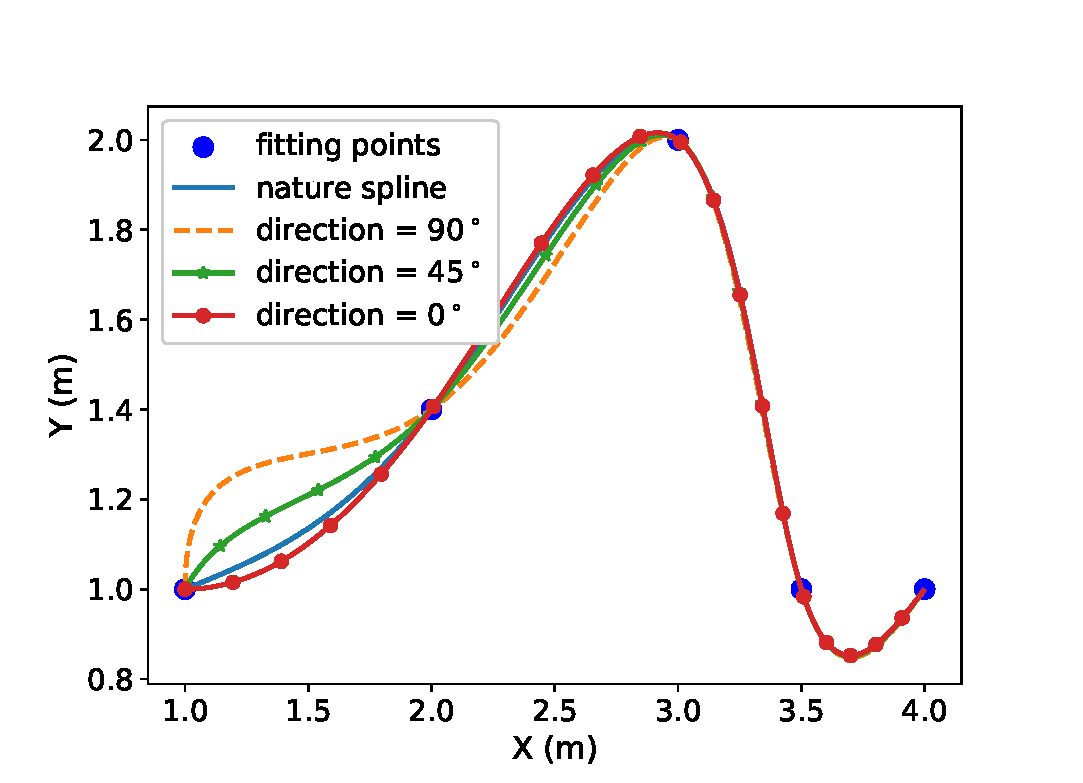
\includegraphics[scale=0.5]{spline.eps}
	\caption{Directional Spline}
	\label{fig_directional_spline}
\end{figure}

Fig.\ref{fig_directional_spline} shows splines with same fitting points but different initial orientations. 

Now we may use to the following parametric curve equation to represent the center-line of the track by simplifying Eq.(\ref{cubic}):
\begin{equation}\label{centerline}
	\mathbf{\Gamma}( \tau)=\sum_{j = 0}^{3}\binom{j}{3}  (\tau-\lfloor \tau\rfloor)^j(1-(\tau-\lfloor \tau \rfloor) )^{3-j}\cdot P_{\lfloor \tau \rfloor j}
\end{equation} 
where $\tau \in [0,N]$ is the parameter of the curve. 

Same approach can be applied to generate the left boundary parametric curve $\mathbf{\Upsilon}(\tau)$ and right boundary $\mathbf{\Psi}(\tau)$ for the racetrack. The waypoints of the left boundary can be derived from the center-line $\mathbf{\Gamma}(\tau)$:
\begin{equation}\label{innerwaypoint}
	W_i^{left} = \min{(n_{\tt max},n_i^{obs})}\cdot  	\mathbf{T}_{l} \frac{\mathbf{\Gamma}'(i)}{\| \mathbf{\Gamma}'(i)\|_2 }
\end{equation} 
where $n_{\tt max}$ is the maximum allowed track offset while $n_i^{obs}$ is the minimum distance from $\mathbf{\Gamma}(i)$ to obstacles along the normal direction, and $\mathbf{T}_{l}=\begin{bmatrix}
	0 & 1 \\
	-1 & 0
\end{bmatrix}$ is the rotation transform matrix.
Same treatment can be applied to get the right boundary $W_i^{right}$ by replacing $\mathbf{T}_l$ with $\mathbf{T}_{r}=\begin{bmatrix}
	0 & -1 \\
	1 & 0
\end{bmatrix}$.
Such treatment approximately makes the vector $\overrightarrow{\mathbf{\Gamma}(\tau)\mathbf{\Psi}(\tau)}$ and $\overrightarrow{\mathbf{\Gamma}(\tau)\mathbf{\Upsilon}(\tau)}$ perpendicular to $\mathbf{\Gamma}'(\tau)$ for any $\tau$.

\begin{figure}
	\centering
	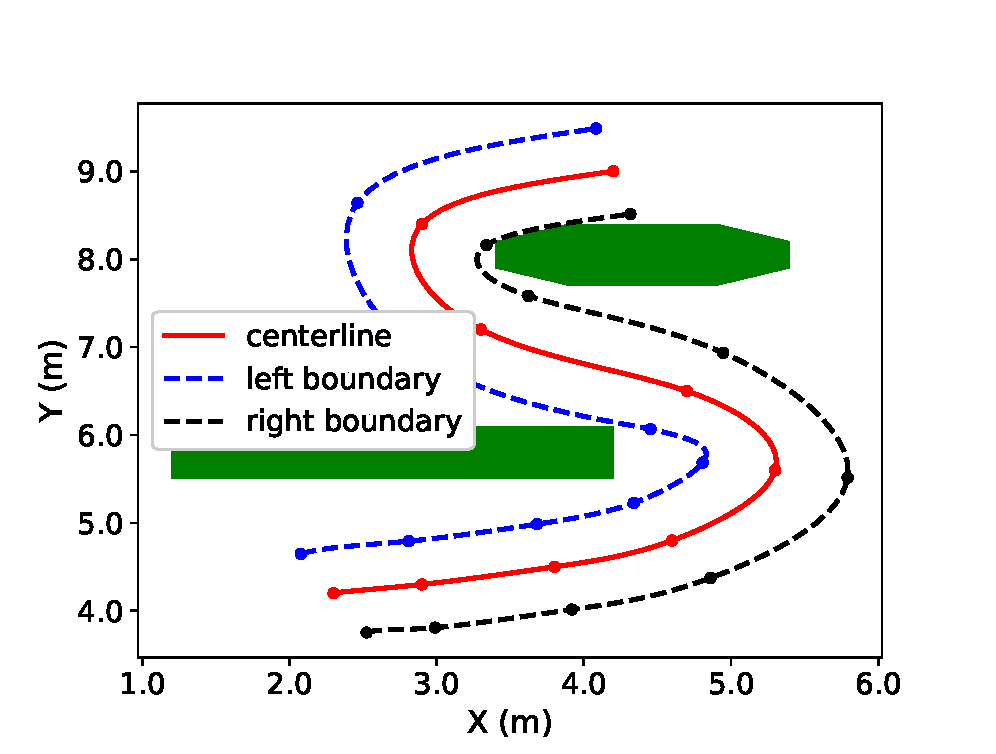
\includegraphics[scale=0.5]{racetrack.eps}
	\caption{A Sample of Racetrack}
	\label{fig_racetrack}
\end{figure}

Fig.\ref{fig_racetrack} show an example of a racetrack.

\subsubsection[optimization]{Trajectory Optimization}\label{trajectoryoptimization}
The purpose of the trajectory optimization is to find the vehicle control input and a feasible path that minimize the total traveling time $T$ of moving the vehicle along the track from start state to the target. As explained in \cite{LOT20147559},\cite{Liniger_2014}, the most effective way to describe the optimization strategy is in the Frenet-Serret(F-S) planar frame, which is shown in Fig.\ref{fig_sn}, where $s$ is the longitudinal displacement along the racetrack, e.g. the traveled length of the racetrack, $n$ is the deviation from the center-line, and $\psi_c$ is the tangent angle of the curve of the center-line. The calculus of the vehicle speed in the dynamics model of Eq.(\ref{2_wheel_model}) in F-S planar frame now is:

\begin{subequations}\label{dynamics_fs}
	\begin{align}
		\dot{s}  & = \frac{v_x \cos(\psi-\psi_c)-v_y \sin(\psi-\psi_c)}{1-n\kappa}
		\label{s_dot}	\\ 
		\dot{n} & = v_x \sin(\psi-\psi_c)+v_y \cos(\psi-\psi_c) 
	\end{align}
\end{subequations}

\begin{figure}[h]
	\centering
	\captionsetup{justification=centering}
	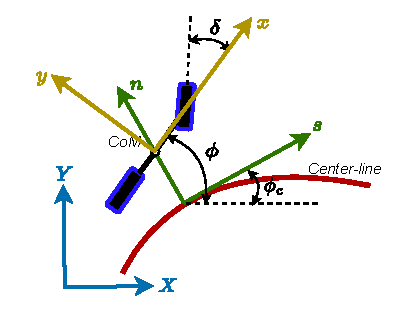
\includegraphics{sn.pdf}
	\caption{Frenet-Serret Frame}
	\label{fig_sn}
\end{figure}

Since the analytical expression of the center-line $\mathbf{\Gamma}$ with respect to $\tau$ is already presented in Eq.(\ref{centerline}), $s$ in Eq.(\ref{s_dot}) can be substituted by $\tau$ with the relations $\frac{ds}{d\tau}=|\mathbf{\Gamma}'(\tau)|$:
\begin{equation}\label{tau_dot}
	\dot{\tau}  = \frac{1}{|\mathbf{\Gamma}'|}\frac{v_x \cos(\psi-\psi_c)-v_y \sin(\psi-\psi_c)}{1-n\kappa}
\end{equation}
Now the state vector is $\boldsymbol{x}=[\tau,n,\psi,v_x,v_y,\omega,\delta]^T$. Let $f(\boldsymbol{x},\boldsymbol{u})$ be the dynamics of the vehicle, the optimal trajectory can be obtained by solving the following OCP:

\begin{subequations}
	\begin{align}
		\min \quad & T\\
		\textrm{s.t.} \quad & \boldsymbol{\dot{x}}=f(\boldsymbol{x},\boldsymbol{u})\\
		\quad &  \boldsymbol{\psi}(\delta,\delta_{dot},d,b)\leqslant 0  \label{ocp_constraints}\\
		\quad &  n^{\tt min}(\tau(t))\leqslant  n\leqslant  n^{\tt max}(\tau(t)) \label{ocp_n_bound}\\
		\quad & \boldsymbol{x}(0)=\bar{\boldsymbol{x}}_0,{\tau(T)}=N,{v_x(T)}=0
		\label{ocp}
	\end{align}
\end{subequations}
where Eq.(\ref{ocp_constraints}) are algebraic inequalities that bound state variable $\delta$ and control variables $\delta_{dot}$, $d$ and $b$. Inequality (\ref{ocp_n_bound}) is used to keep the vehicle traveling in the range of the racetrack, where $n^{\tt min}(\tau(t)) = -\|\mathbf{\Gamma}(\tau(t))-\mathbf{\Psi}(\tau(t))\|$ and $n^{\tt max}(\tau(t)) = \|\mathbf{\Gamma}(\tau(t))-\mathbf{\Upsilon}(\tau(t))\|$. 
The OCP (\ref{ocp}) is hard to solve due to the high non-linearity of $\mathbf{\Gamma}$ and the presence of inequality constraint(\ref{ocp_constraints}). The following two treatments are applied to increase the chance of getting an optimal solution.
\begin{enumerate}
	\item Discrete the whole racetrack to $N^c$ segments with equivalent length.
	\item Convert the inequality constraint (\ref{ocp_n_bound}) to soft constraints used as a penalty term in objective function, the value of which is small when $n^{\tt min}\leqslant  n\leqslant  n^{\tt max} $ but increases rapidly if $n$ exceeds the boundaries. 	 
\end{enumerate}

We use the exponential as the penalty term and let $s(\overline{\tau}_{i+1})-s(\overline{\tau}_{i})=s(\overline{\tau}_{i})-s(\overline{\tau}_{i-1})$ for $i \in [1,N^c]$, the OCP(\ref{ocp}) can be rewritten as:
\begin{subequations}
	\begin{align}
		\min \quad & \sum_{i = 1}^{N^{c}}\left(\varDelta t_i + \gamma\left(e^{\lambda(n^{\tt min}_i-n_i) }+e^{\lambda(n_i-n^{\tt max}_i) }\right)\right)\\
		\textrm{s.t.} \quad & \boldsymbol{x}_{i+1}=\varDelta t_i f(\boldsymbol{x}_i,\boldsymbol{u}_i)\\
		\quad &  \boldsymbol{\psi}(\delta_i,\delta^{dot}_i,d_i,b_i)\leqslant 0 \\
		\quad & \tau_i=\bar{\tau}_i \\
		\quad & \boldsymbol{x}_0=\bar{\boldsymbol{x}}_0,v^x_{N^c+1}=0
		\label{ocp_refine}
	\end{align}
\end{subequations}
where $\gamma$, $\lambda$ are weights, $\varDelta t_i$ is the traveling time of $i$th segment. Since $\overline{\tau}_{i}$ is known, other parameters, e.g. $n^{\tt min}_i,\psi^c_i$, related to $\tau_{i}$ can be gained, which simplifies the calculation of the OCP. 

\subsection{Trajectory Tracking(Motion Control)}
An NMPC shown in Eq.(\ref{trajectorytrack}) is applied for trajectory tracking. Different from trajectory generating process, Cartesian frame rather than F-S frame is used to simplify the computational process. The reference trajectory can be represented by $\boldsymbol{y}=tr(t),t \in [0,T]$, where $T$ is the optimal time of the trajectory and $\boldsymbol{y}$ is the vehicle state in F-S frame. We also can map the traveling distance to traveling time as $t=tr^{-1}(\boldsymbol{y})$. For a vehicle state $\widetilde{\boldsymbol{x}_0}$ in Cartesian frame, whose corresponding state in F-S frame is $\widetilde{\boldsymbol{y}_0}$, we first get the reference time $t_0=tr^{-1}(\widetilde{\boldsymbol{y}_0})$, and divide the time span $[t_0,t_0+T]$ to $k+1$ reference time points. Then get a set of reference states $\widetilde{\boldsymbol{y}_0},\widetilde{\boldsymbol{y}_1},...,\widetilde{\boldsymbol{y}_k}$ and $\widetilde{\boldsymbol{x}_0},\widetilde{\boldsymbol{x}_1},...,\widetilde{\boldsymbol{x}_k}$ via $\boldsymbol{y}=tr(t)$
\begin{equation}
	\label{trajectorytrack}
	\begin{aligned}
		\min \quad & \sum_{i = 0}^{N}\left((\boldsymbol{x}_i-\widetilde{\boldsymbol{x}_i})^TQ(\boldsymbol{x}_i-\widetilde{\boldsymbol{x}_i}) + (\boldsymbol{u}_i-\widetilde{\boldsymbol{u}_i})^TR(\boldsymbol{u}_i-\widetilde{\boldsymbol{u}_i})\right)\\
		\textrm{s.t.} \quad & \boldsymbol{x}_{i+1}=\varDelta t_i f(\boldsymbol{x}_i,\boldsymbol{u}_i)\\
		\quad &  \boldsymbol{\psi}(\delta_i,\delta^{dot}_i,d_i,b_i)\leqslant 0 \\
		\quad & \boldsymbol{x}_0=\widetilde{\boldsymbol{x}}_0
		\\
	\end{aligned}
\end{equation}
where $Q$ and $R$ are weight matrices for state and control input, respectively.

\subsection{The Ref-iSST algorithm and Global Route}
The $\tt Ref-iSST$ path planning algorithm is developed for another project - the microfluidic system that consists of $N \times N$ electrode arrays. The electrodes are independently and intermittently powered with a DC voltage. The electrode arrays are on the substrate and covered by a fluid that contains a dilute concentration of micro- or nanowires. The motion of the wires is guided by the electrical field wirelessly. One of the biggest limitations of wireless external actuation is its global and coupled influence in the workspace, which limits the capability to robustly manipulate multiple agents independently and simultaneously.

A reference trajectory is required to control the wires from their random positions to the destinations. By applying the Bi-iSST algorithm, we find the wires are prone to travel along the edge of the cell formed by the nearest $2 \times 2$ electrodes. The Ref-iSST algorithm is developed based on this phenomenon. First an optimal global reference trajectory is generated by scheduling the electrode array states. Then an algorithm is applied to force the wires following the global reference trajectory. 

\subsubsection{Global Route}
The global routing here means scheduling a sequence of
turning on and off of the electrodes to form the reference trajectory. Because the electric field acting on an agent is inversely proportional to the square of the distance to the electrodes, only the neighboring electrodes have significant effects on the motion of the agents. The algorithm is based on the following two assumptions:
\begin{enumerate}	
	\item An agent can only be located on an electrode and count one-step if there is any agent	that moves from one electrode to a neighboring electrode.
	\item In one step, an agent can go to any of the neighboring electrode by turning on the electrode where the agent locates and turning off the destination one. Or the agent can be UNMOVED by turning on the electrode where the agent locates.
\end{enumerate}
For an $N \times N$ electrodes microfluidic device with $m$ micro agents, there are $N^{2m}$ states in total. A value $s = \sum_{1}^{m}(r_iN^i+c_iN^{i-1})$ is used to indicate a state, where $r_i$ and $c_i$ are the row and the column indices of the electrode where the $i$th agent locates. 

Similar to the MDPs, a pre-constructed transition matrix $\textbf{M}_t \in \mathcal{R}^{N^{2m} \times N^{2m}}$ is used to indicate the transition between two states. Each element in the MDP transition matrix represents the state transition probability. It can be simplified to zero or one in global routing, e.g. $\textbf{M}_{ij} \in \{0,1\}$, where $\textbf{M}_{ij} = 1$ represents the $i$th state can be reached from $j$th state within one step.
By monitoring the value of $j$th row of the vector $S_n$ in a continued multiplication $S_n =\textbf{M}S_{n-1}$, we can obtain the minimum steps from a start configuration to a target when $S_n(s_t)\neq 0$. $j$ corresponds the target state and $S_0$ is the initial vector whose $s_0$th element representing the start state is set to one while others are zero, e.g. $S_0(i) = 1$ for $i=s_0$ and $S_0(i) = 0$ for $i \neq s_0$.

The GBTM (Global Routing With Transition Matrix) algorithm uses a tree to schedule the global trajectory as shown in Algorithm~\ref{globalroute}. First the initial state is set as the root of the tree and set $\mathbb{P} $ can be considered as the collection of tree leaves. In Line 2, we get the minimum steps from the start to the target states, i.e., the depth of the tree as described above. The feasible states of the next step for each leaf(Lines 5-6) can be obtained via the transition matrix. To reduce the redundancy of the tree, the states whose minimum estimated steps to target exceeds $n_{\tt min}-k$ are removed, where $k$ is the depth of the current leaf. Because a new state may be conducted from different leaves, only the leaf with the best quality will be selected as the parent of the new state. The quality of a node is defined as $\sum_{1}^{k} \sum d_m(e_i,e_j)$, where $d_m$ is the Manhattan distance of the two turned ``on" electrodes $e_i$ and $e_j$, $i, j=1,\cdots, N^2$ and $i\neq j$ for each step. In Line 9-11, the leaves at $(k-1)$th step with no child are trimmed. Set $\mathbb{Y}$ contains only one leaf that is the same as $\textbf{q}_{\tt t}$ at the last step, which guarantees the existence of the path from the start to the target state.

\begin{algorithm}[ht!]
	\caption {${{\tt GRTM}}$}
	\label{globalroute}
	% \Input{ $\mathcal{G}, \mathcal{R}, p$}
    % \hspace*{\algorithmicindent} \textbf{Output}  $\mathcal{\pi}$
	% \Input{ $\textbf{q}_{\tt s},\textbf{q}_{\tt t}$}
	% \Output{ $\mathcal{\pi}$}
	\DontPrintSemicolon
	\SetAlgoVlined
	\BlankLine	
	$\mathcal{T}  \gets \mathtt{init}(q_{\tt s}) $,	$\mathbb{P}  \gets \{q_{\tt s}\} $\;
	$n_{\tt min} \gets \mathtt{Find\_Minimum\_Steps}(\textbf{q}_{\tt s},\textbf{q}_{\tt t}) $\;	
	
	\For{$k \gets 1$ to $n_{\tt min}$}{
		$\mathbb{Y} \gets \emptyset$ \;
		\ForEach{$q \in \mathbb{P}$}{
			$\mathbb{Y} \gets \mathbb{Y} \cup \mathtt{Get\_Next\_States}(q,n_{\tt min}-k)$
		}
		\ForEach{$y \in \mathbb{Y}$}{
			$ \mathtt{Set\_Best\_Parent}(y,\mathcal{T},\mathbb{P})$
		}
		\ForEach{$q \in \mathbb{P}$}{
			\If{$\mathtt{Has\_No\_Child}(q)$}{
				$\mathtt{Remove\_From\_Tree}(\mathcal{T},q)$
			}
		}
		$\mathbb{P}  \gets \mathbb{Y}$
		
	}	
	$\mathcal{R} \gets \mathtt{Get\_Global\_Route}(\mathcal{T})$	
\end{algorithm}



It is infeasible to store the whole transition matrix even though the matrix is in sparse format because its size grows exponentially with the number of the agents. Such kind of matrices can be constructed by two low-dimension control transition matrices $\textbf{D}$, whose structure is similar to the transition matrices $\textbf{M}$ while a control matrix $\textbf{C} \gets \mathbb{R}^{N \times N}$ is used to represent the none-zero element. Each element of the matrix $\textbf{C}$ reflects the state of an electrode. For instance, 1, -1, and 0 represent ``on",``off", and ``free" states, respectively, where ``free" refers to the state of the electrode that does not affect the transition process. The product of the control matrices is defined as
\begin{equation}
	{\textbf{C}_1 \cdot \textbf{C}_2 } = \left\{\begin{matrix}
		0, {\tt if \ } \textbf{C}_1 {\tt \ and\ } \textbf{C}_2 {\tt\  not\ compatible}, \\1, {\tt if \ } \textbf{C}_1 {\tt \ and\ } \textbf{C}_2 {\tt\  compatible}.
	\end{matrix}\right.
	\label{controltransitiondot}
\end{equation}
For the previous instance, $\textbf{C}_1 \cdot \textbf{C}_2 = 0$  (not compatible) if any of $\textbf{C}_1(i,j) \cdot \textbf{C}_2(i,j) =-1$, otherwise $\textbf{C}_1 \cdot \textbf{C}_2 = 1$. 


For a state $s$ with $m$ agents, divide the state into two sub-configurations with $m=m_1 + m_2$ and $s = s_1N^{2m_2}+s_2$. Then apply the matrix multiplication $\widetilde{\textbf{D}^s} = \textbf{D}_1^{s_1} \times (\textbf{D}_2^{s_2})^T$, where $\textbf{D}_i^{s_i}(i=1,2)$ are the control transition vectors for the $m_i$ agent's configuration at state $s_i$ ($s_i$th column of matrix $\textbf{D}_i$), and $\widetilde{\textbf{D}^s}(i,j) = \textbf{D}_1^{s_1}(i) \cdot \textbf{D}_2^{s_2}(j)$. Finally, resize $\widetilde{\textbf{D}^s}\in \mathcal{R}^{N^{2m_1} \times N^{2m_2}}$ to $\textbf{D}^s \in \mathcal{R}^{N^{2(m_1+m_2)} \times 1}$ to get the transition vector for $m$ micro agents at the state $s$.

\begin{figure}[thb!]

	\centering
	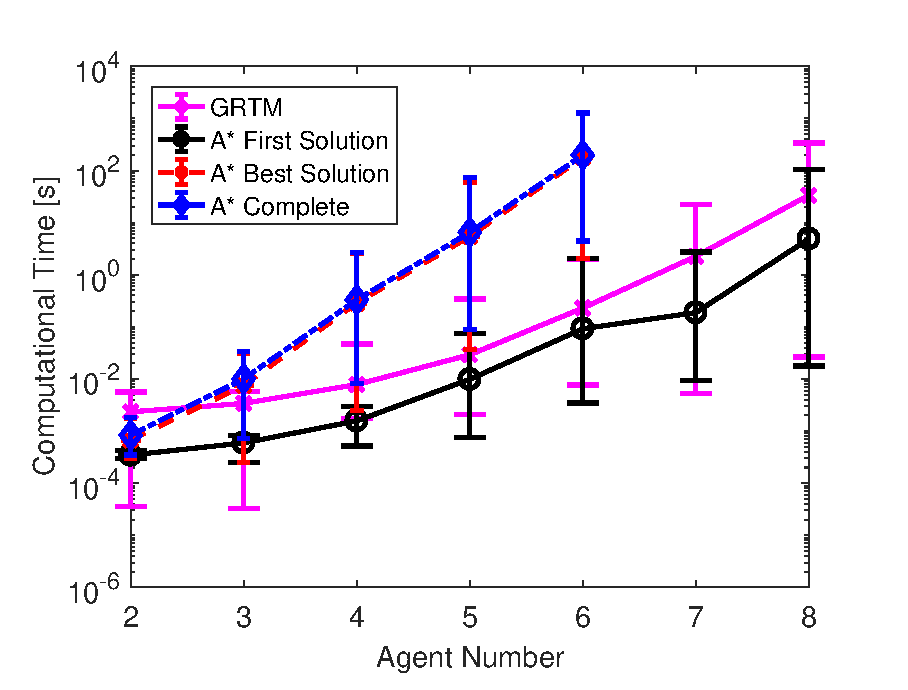
\includegraphics[scale=0.6]{globalroute}
	\caption{Computational cost for the global routing algorithms. }
	\label{globalroutefig}
\end{figure}


The comparison of the global routing algorithm and A* is shown in Fig.~\ref{globalroutefig}. The A$^*$ First Solution is the computational time of the very first path found by the A$^*$-based global routing algorithm. The curve of A* Best Solution represents the computational time of finding the optimal path and A* complete illustrates the computational time of the A$^*$-based global routing algorithm that exhaustively explores all the possible actions. From the comparison, it is obvious that the proposed GRTM algorithm outperforms the A$^*$-based global routing algorithm in the computation complexity. Such a performance gap becomes apparent as the agent number increases. However, the A*-based global routing algorithm can quickly find an initial solution though the solution quality is far worse than the optimal one. 

\subsubsection{The ${{\tt Ref}}$-$\tt iSST$ algorithm}

 
The most significant difference between the $\tt Ref$-$\tt iSST$ algorithm and $\tt Bi$-$\tt iSST$ is that the heuristic value is estimated using the waypoints rather than the single target state in $\tt Ref$-$\tt iSST$. The waypoints are on the global reference trajectory generated by GRTM. Because the waypoints locate nearer to the current state, the heuristic value becomes more accurate. Therefore, the algorithm converges to the optimal solution much faster.

Algorithm~\ref{refisst} gives the basic structure of the $\tt Ref$-$\tt iSST$ algorithm. In Line 1, we first generate a global reference trajectory $\mathcal{R}$, the cost of which underestimates the optimal solution. A new {$\tt Ref\_Search\_Selection$} process (Line 4) is shown in Algorithm~\ref{searchselection}. 
In the node selection process, we not only employ $\tt iSST$-like search selection, but also keep a certain probability, $p$, to select vertices near the reference that prioritizes the propagation along the reference trajectory (Lines 5-6 in Algorithm~\ref{searchselection}). Similar as the $\tt SST$ algorithm, the ${\tt Best\_Near}$ process is used to select the least-cost vertex to the reference trajectory.



\begin{algorithm}[ht!]
	\caption {${{\tt Ref}}$-${{\tt iSST}}$}
	\label{refisst}
	%\Input{ $\textbf{q}_{\tt s},\textbf{q}_{\tt t}$}
	%\Output{ ${\sigma}^*$}
	\DontPrintSemicolon
	\SetAlgoVlined
	\BlankLine
	$\mathcal{R} \gets \tt{GRTM}(\textbf{q}_{\tt s},\textbf{q}_{\tt t}) $\;
	$\mathcal{G},\mathbb{W}\  \gets \tt{init}(\textbf{q}_{\tt s});\mathbb{E}, \mathbb{P}\gets \emptyset $\;
	\For{$m\ \text{iterations}$}{	
		$x_{\tt selected} \gets \mathtt{Ref\_Search\_Selection}(\mathcal{G}, \mathcal{R})$\;
		
		$\mathbb{X}_{\tt temp} \gets \mathtt{Blossom}(\mathcal{R},x_{\tt selected},l)$
		
		\ForEach{$x \in \mathbb{X}_{\tt temp}$}
		{
			
			\If {$ {\tt not } \  \mathtt{Collision\_Free}(\overline{x_{\tt selected}\rightarrow x})$}{
				\Continue
			}
			\If {$ {\tt not}\  \mathtt{Local\_Best\_SST}(x,\mathbb{W},\delta_{\tt s})$ }{
				\Continue
			}
			$\mathcal{G} \gets \mathcal{G} \cup \{x\}$,
			$\mathbb{E} \gets \mathbb{E} \cup \{\overline{x_{\tt curr}\rightarrow x}\}$\;
			
			$\mathtt{Prune\_Dominated\_Nodes\_SST}(\mathcal{G},\mathbb{W},x)$\;
			\If {$\mathtt{distance}(x,q_{\tt t})<\delta{_{\tt watch}}$}
			{
				$\mathbb{P} \gets \mathbb{P} \cup \{x\}$\;
				
			}
		}
	}
	$\mathcal{\pi} \gets \mathtt{Get\_Best\_Trajectory}(\mathcal{G})$	
\end{algorithm}

Algorithm~\ref{refisst} gives the basic structure of the $\tt Ref$-$\tt iSST$ algorithm. The global reference trajectory $\mathcal{R}$ is generated under an ideal model, so the cost underestimates the optimal solution. Not only does the propagating node selection process {$\tt Ref\_Search\_Selection$}(Lines 4) employ $\tt iSST$-like search selection, it also keeps a certain probability, $p$, to select vertices near the reference that prioritizes the propagation along the reference trajectory.
The $\tt Blossom$ procedure (Line 5) generates a set $\mathbb{X}_{\tt temp}$ containing $l$ temporary nodes by applying a series of propagations originated at $x_{\tt selected}$ with random control inputs. 
The $l$ temporary nodes are prioritized according to the quality function shown in Eq.~(\ref{quality}). Each temporary node is tested to avoid collision (Line 7) and keep sparsity (Line 9). %The collision-free active vertex in the sparse region with the best quality is continued to propagate, and the other nodes are classified into the open set for future propagation.

\begin{equation}
	{\tt quality}(x) = 
		\frac{\exp(-k\cdot{a}\cdot{\frac{|c-c_{\tt max}|}{\max(c,c_{\tt max})})}}{{\tt distance}(x,x_{\tt ref})},
	\label{quality}
\end{equation}
Where $c$ is the cost of the vertex $x$ and $c_{\tt max}$ is the total cost of the reference trajectory. $x_{\tt ref}$ is the estimated state in the reference trajectory corresponding to $c$ and the target state is selected as the reference state if the vertex's cost exceeds the total cost of the reference trajectory. Parameter $a$ represents the weight of cost in the quality measure and $k$ is a degrading factor with respect to $c$, where $k=1$ for $c<c_{\tt max}$ and $k>1$ for $c>c_{\tt max}$. The quality function aims to prioritize the vertex whose state is closer to the estimated state with the same cost in the reference trajectory. By setting $k>1$ for $c>c_{\tt max}$, the temporary state around the target state with less cost is prioritized.

\section{Research Plan}
The motion controller works well for low speed scenario. However, when the speed reaches around 25 m/s in the simulation environment, the vehicle can't follow the reference trajectory, especially for the region with sharp turns. The reasons causing such failure may be:
\begin{enumerate}
	\item the description of the dynamics model is not precise. Some degrees of freedom, like pitch and roll, are ignored. 
	\item the computational speed can't catch up with the vehicle speed. Different from the traditional feedback controller that will give an output instantly, the output of MPC has a time lag in recent PC configuration since it has to solve an optimization problem. We set this time lag to 0.1 second and the initial state $\boldsymbol{x}_0$ is estimated in Eq.(\ref{trajectorytrack}).  
\end{enumerate}

We are going to work on these two factors, trying to increase the maximal speed that can be tracked.
% \begin{algorithm}[ht!]
% 	\caption {${{\tt Ref}}$\_${{\tt Search}}$\_${{\tt Selection}}$}
% 	\label{searchselection}
% 	%\Input{ $\mathcal{G}, \mathcal{R}, p$}
% 	%\Output{ $x_{\tt selected}$}
% 	\DontPrintSemicolon
% 	\SetAlgoVlined
% 	\BlankLine
	
% 	$u \gets {\tt Uniform}([0,1])$ \;
% 	\If{$u>p$}{
% 		$x_{\tt selected} \gets \mathtt{iSST\_Search\_Selection}(\mathcal{G})$ \;
		
% 	}
% 	\Else{
% 		$x_{\tt ref} \gets \tt {Random\_Select}(\mathcal{R})$\;
% 		$x_{\tt selected} \gets {\tt Best\_Near}(\mathcal{G},x_{\tt ref},\delta_{\tt BN})$\;
		
% 	}
% 	\Return{$x_{\tt selected}$}	
% \end{algorithm}
\bibliographystyle{IEEEtran}
\bibliography{bib/xilin_bib_modified.bib}

\end{document}